\documentclass[fleqn,12pt,a4paper]{report}
\usepackage{biblatex}
\usepackage{cmap}
\usepackage[T2A]{fontenc}
\usepackage[utf8]{inputenc}
\usepackage[english,ukrainian]{babel}
\usepackage[fleqn]{amsmath}
\usepackage{amsthm}
\usepackage{latexsym}
\usepackage{amssymb}
\usepackage{amscd}
\usepackage{epsfig}
\usepackage{graphics}
\usepackage{longtable}
\usepackage{indentfirst}
\usepackage{comment}
\usepackage{enumerate}
\usepackage{color}
\usepackage{xurl}
\usepackage[labelsep=period]{caption}
\usepackage[
    pdftex,
    colorlinks,
    linkcolor=blue,
    citecolor=red,
    urlcolor=blue,
    hyperindex,
    plainpages=false,
    bookmarksopen,
    bookmarksnumbered,
    unicode
]{hyperref}
\usepackage{setspace}
\usepackage[
    textwidth=160mm,
    textheight=230mm,
    headheight=16pt,
    includehead,
    includefoot
]{geometry}
\usepackage{fancyhdr}
\usepackage[small,center]{titlesec}
\usepackage{zref-totpages}
\usepackage{totcount}
\usepackage{graphicx}

\addbibresource{theorems.bib}

\setstretch{1.20}

\pagestyle{fancyplain}
\fancyhf{}
\fancyhead[R]{\thepage}
\renewcommand{\headrulewidth}{0pt}

\setlength{\topmargin}{0mm}
\setlength{\parindent}{7.0mm}
\setlength{\evensidemargin}{0mm}
\setlength{\oddsidemargin}{10mm}

\titlespacing{\chapter}{0pt}{15pt}{19pt}
\titleformat{\section}[hang]{\filright\bfseries\Large}{\thesection.}{6pt}{}
\titlespacing{\section}{\parindent}{15pt}{12pt}

\newtotcounter{refnum}
\AtEveryBibitem{\stepcounter{refnum}}

\theoremstyle{plain}
\newtheorem{theorem}{Теорема}
\theoremstyle{definition}
\newtheorem{definition}{Означення}

\numberwithin{equation}{chapter}
\numberwithin{figure}{chapter}
\numberwithin{table}{chapter}
\numberwithin{footnote}{chapter}
\numberwithin{figure}{chapter}
\numberwithin{theorem}{chapter}
\numberwithin{definition}{chapter}

\begin{document}
    \begin{center}
        \Large \textbf{Анотація}
    \end{center}
    \noindent
    \textbf{Петраківський Д.О.} \textbf{<<Автоматизована система модерації електронного каталогу>>}, Кваліфікаційна
    робота на здобуття освітнього ступеня <<магістр>> за спеціальністю 122 Комп'ютерні науки, Київський академічний
    університет, Київ, 2024, сторінки --- \ztotpages, джерела --- \total{refnum}.

    \bigskip
    \noindent
    \textbf{ACM:} I.2.7, I.2.10.

    \bigskip
    \noindent
    \textbf{Ключові слова:} модерація вмісту, ієрархічна класифікація, широкомасштабна класифікація, дизбалансна
    класифікація.

    \newpage
    \tableofcontents

    \newpage

    \chapter*{Перелік умовних позначень}\label{ch:conventions}
    \addcontentsline{toc}{chapter}{Перелік умовних позначень}

    \bigskip
    \begin{tabular}{ll}
        $\bigoplus$ & конкатенація тензорів         \\
        $\times$    & поелементне множення тензорів \\
        $\sigma$    & софтмакс
    \end{tabular}

    \newpage

    \listoffigures
    \addcontentsline{toc}{chapter}{Перелік ілюстрацій}

    \newpage

    \chapter*{Вступ}\label{ch:introduction}
    \addcontentsline{toc}{chapter}{Вступ}

    На полі систем модерації є чимало попередніх досліджень.
    Наприклад, Nguyen~\cite{Nguyen2022} пропонує метод очищення зразків з неправильними категоріями, а також нейронну
    мережу з використанням CNN~\cite{Lecun1998} та BiLSTM~\cite{Schuster1997} для категоризації товарів за назвами.
    У рамках нашої задачі доводиться оперувати на порядки більшою кількістю категорій та предметів, ніж було
    використано в наведеному підході, тому ми віддали перевагу ручній модерації вибірки з поєднанням евристик для
    прискорення маркування.

    Значно ближчим до наших умов є рішення Zhang~\cite{Zhang2021}, яке передбачає ієрархічний класифікатор.
    Дана робота використовує виключно текстові ознаки товарів, але до заголовків додаються описи й характеристики.
    Векторизатором обрано багатомовну модель BERT~\cite{devlin-etal-2019-bert}.
    Для наших умов цей підхід не підійшов через порівняно громіздку систему обчислень, яку складно підтримувати з
    поточним навантаженням, а також відсутність картинок, як репрезентативної ознаки.

    Ще одним релевантним методом поділилися фахівці Shopify~\cite{shopify2020}, які аналогічно застосували текстові
    поля для побудови конкатенованих векторів товарів.
    Вони використали TF-IDF для обробки назв, описів, постачальників та тегів, після чого застосували логістичну
    регресію, яка замість $N$ окремих моделей для $k$ класів має єдині ваги з $Nk$ комірками.

    На початку дослідження електронний магазин вже використовував автоматизовану систему модерації з евристичним
    алгоритмом, який базувався на словниках для нормалізації від pymorphy2~\cite{pymorphy2} та перевірки правопису від
    hunspell~\cite{hunspell}, а також моделі Bag-of-Words (BOW).

    \newpage


    \chapter{Запропонований алгоритм}\label{ch:chaper1}


    \section{Архітектура моделі}\label{sec:section1.1}

    Векторизатором для текстових даних виступив USE~\cite{yang-etal-2020-multilingual}, а для зображень --- \\
    CAFormer, одна з реалізацій MetaFormer~\cite{10304335}.
    Обмеження векторизатора назв --- не більше 256 токенів~[\ref{def:definition2.1}] у реченні.

    \noindent
    \begin{figure}[ht]
        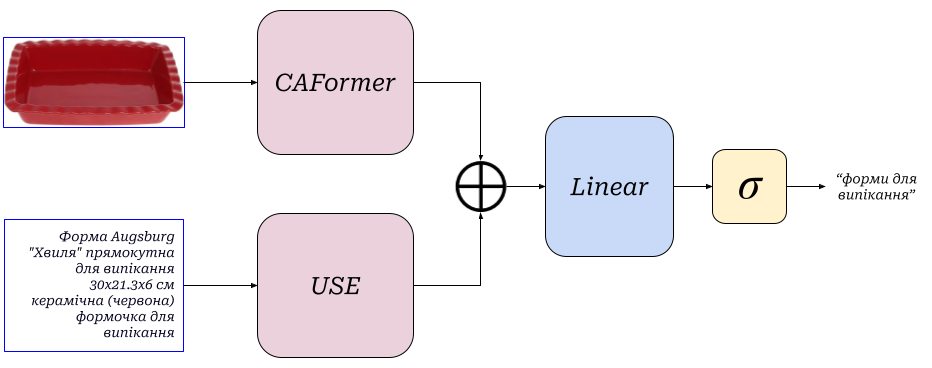
\includegraphics[width=\textwidth]{images/catify-concatenated-model}
        \caption{Схема роботи класифікатора.}
    \end{figure}

    \newpage


    \section{Дані товарів}\label{sec:section1.2}

    Тут буде трішки про поля товару --- назву, головне фото, ключові слова, опис, теги й т.д.
    Для зображення класів-дублів можна скористатися UMAP-проєкцією~\cite{mcinnes2018umap-software}.

    \noindent
    \begin{figure}[ht]
        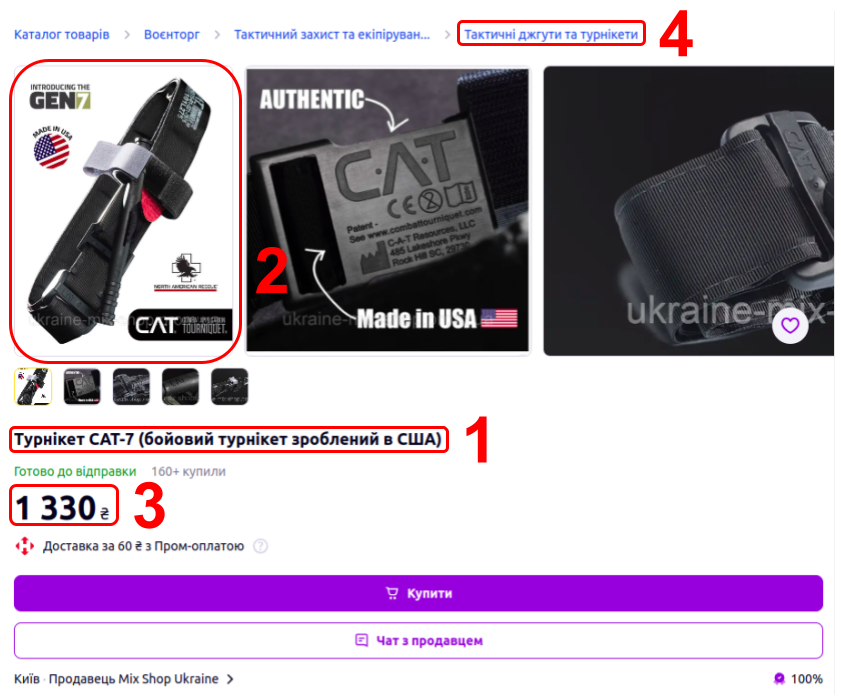
\includegraphics[width=\textwidth]{images/catify-product}
        \caption{Картка товару.}
    \end{figure}

    \newpage


    \section{Дерево каталогу}\label{sec:section1.3}

    Класи товарів зібрані в таксономію, яка за своєю структурою є орієнтованим ациклічним графом.
    Кожен предмет належить одній і тільки одній категорії.

    \noindent
    \begin{figure}[ht]
        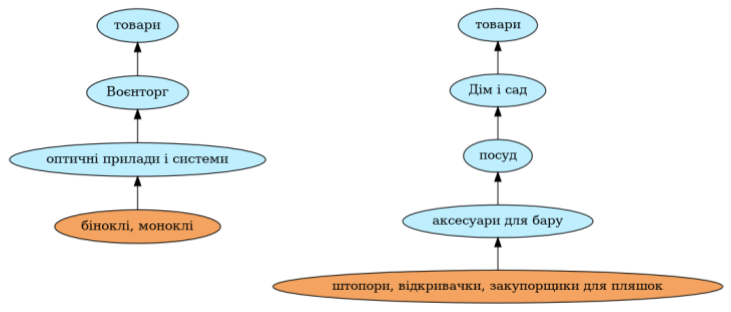
\includegraphics[width=\textwidth]{images/catify-hierarchies}
        \caption{Приклади категорійних ієрархій.}
    \end{figure}

    \noindent
    \begin{figure}[ht]
        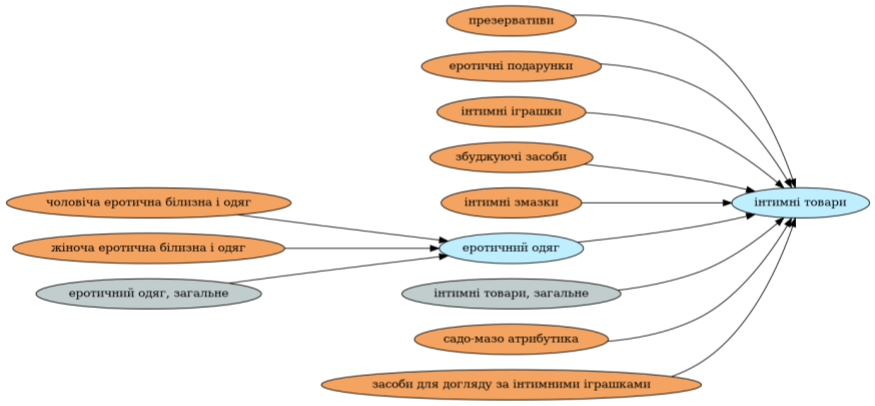
\includegraphics[width=\textwidth]{images/catify-category-tree}
        \caption{Фрагмент дерева категорій.}
    \end{figure}

    \newpage


    \section{Експерименти}\label{sec:section1.4}

    Тут буде інформація про етапи розвитку класифікатора та порівняльні метрики.

    \noindent
    \begin{figure}[ht]
        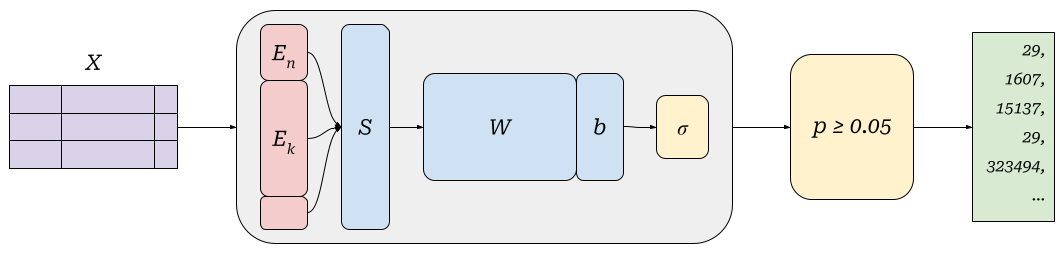
\includegraphics[width=\textwidth]{images/catify-linear-model}
        \caption{Лінійна модель.}
    \end{figure}

    \noindent
    \begin{figure}[ht]
        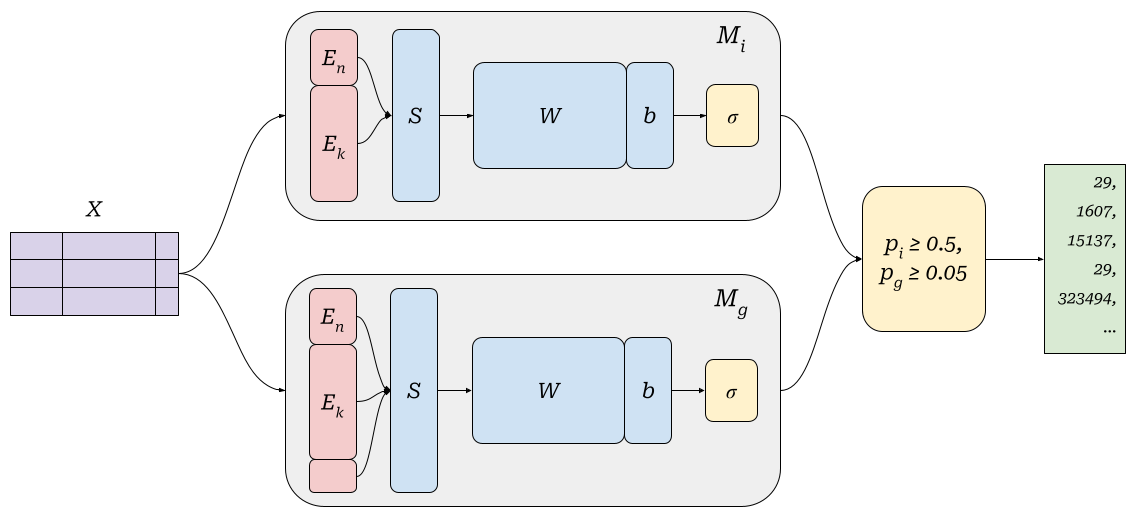
\includegraphics[width=\textwidth]{images/catify-cascading-model}
        \caption{Каскадна модель.}
    \end{figure}

    \newpage


    \chapter{Розгортання}\label{ch:chaper2}


    \section{Канали надходження даних}\label{sec:section2.1}

    Тут буде інформація про мікросервісну архітектуру й пайплайн оновлення.


    \section{Використані технології}\label{sec:section2.2}

    У цьому розділі будуть перелічені інструменти й програмні бібліотеки, використанні при розробці й апробації
    системи, а також наведене обґрунтування саме такого вибору.
    А поки пропонуємо поглянути на теореми.

    \begin{theorem}
        \label{the:theorem2.1}
        Нехай $X_{k}$ --- послідовність взаємно незалежних випадкових величин з однаковими розподілами, які мають
        скінченне математичне сподівання $\mu = E(X_{k})$ та скінченну дисперсію $\sigma ^ 2 = D(X_{k})$.
        Нехай $S_{n} = X_{1} + \dots + X_{n}$.
        Тоді
        \[\sqrt{n} \biggl(\frac{S_{n}}{n} - \mu \biggr) \xrightarrow{n} N \bigl(0, \sigma ^ 2 \bigr),\]
        а для довільних фіксованих $\alpha, \beta \ (\alpha < \beta)$ справедливо
        \[P\left\{\alpha < \frac{S_{n} - n \mu}{\sigma n ^ {1 / 2}} < \beta \right\} \to \Phi(\beta) - \Phi(\alpha),\]
        де $\Phi(x)$ --- нормальна функція розподілу.
    \end{theorem}

    \begin{definition}
        \label{def:definition2.1}
        Токен --- об'єкт, що утворюється із лексеми в процесі лексичного аналізу.
        У прикладному програмуванні поняття токена та його лексема можуть не розрізнятися.
        Шаблон токена --- формальний опис класу лексем, які можуть утворити даний тип токена.
    \end{definition}

    \newpage

    \chapter*{Висновки}
    \addcontentsline{toc}{chapter}{Висновки}

    Тут буде повторення наукової новизни та подальших планів розвитку.

    \printbibliography[title={Список використаних джерел},heading=bibintoc]
\end{document}
